% Appendix Template

\newcommand{\major}{3}
\newcommand{\minor}{4}

\newcommand{\undPrefix}{\major_\minor}
\newcommand{\dotPrefix}{\major.\minor}
\newcommand{\scoPrefix}{\major-\minor}
\newcommand{\filePrefix}{\undPrefix}

% \chapter{Results of experiment 1.1} % Main appendix title
\chapter{Results of experiment \dotPrefix} % Main appendix title

% \label{Appendix1-1} % Change X to a consecutive letter; for referencing this appendix elsewhere, use \ref{AppendixX}

\label{Appendix\scoPrefix} % Change X to a consecutive letter; for referencing this appendix elsewhere, use \ref{AppendixX}

These experiments are discussed \hyperref[disc:h3]{here}
\begin{figure}[ht]
  \centering
  \begin{subfigure}[t]{0.5\linewidth}
    % \centering\captionsetup{width=.8\linewidth}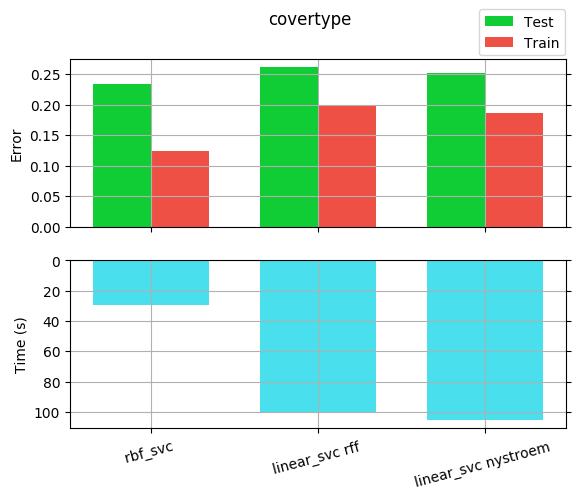
\includegraphics[width=\imgscale\linewidth]{Figures/1_1/covertype}
    \centering\captionsetup{width=.8\linewidth}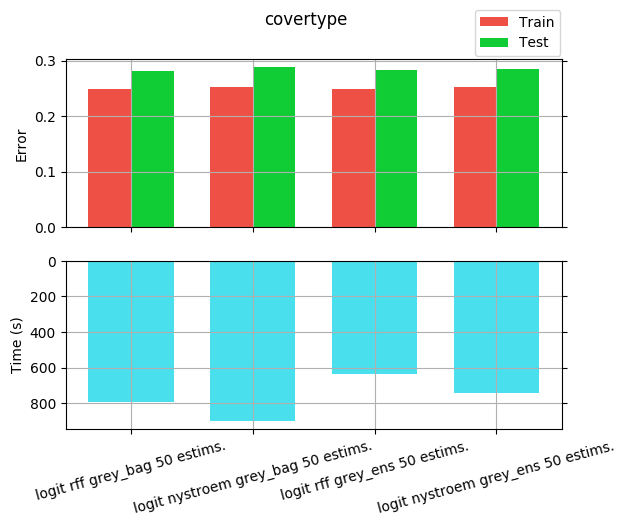
\includegraphics[width=\imgscale\linewidth]{Figures/\filePrefix/covertype}
    \caption{Exp. 3.4 with Covertype. Black Box Models with Support Vector Machine. There is not much difference between Box Models}
    \label{fig:\undPrefix_covertype}
  \end{subfigure}%
  \begin{subfigure}[t]{0.5\linewidth}
    \centering\captionsetup{width=.8\linewidth}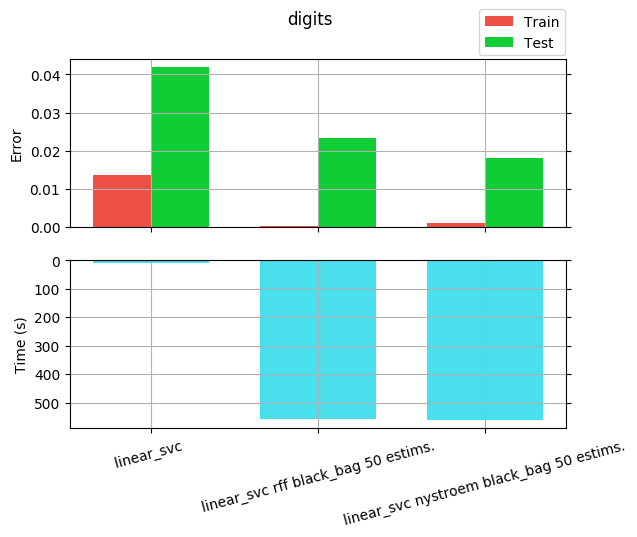
\includegraphics[width=\imgscale\linewidth]{Figures/\filePrefix/digits}
    \caption{Exp. 3.4 with Digits. Black Box Models with Support Vector Machine. There is not much difference between Box Models}
    % \label{fig:1_1_digits}
    \label{fig:\undPrefix_digits}
  \end{subfigure}
\end{figure}


\begin{figure}[ht]
  \centering
  \begin{subfigure}[t]{0.5\linewidth}
    \centering\captionsetup{width=.8\linewidth}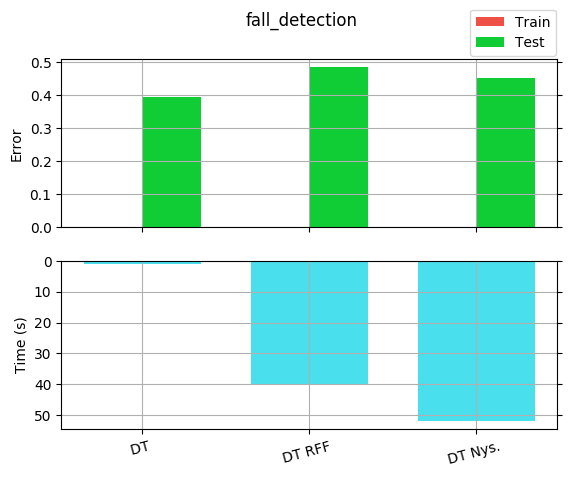
\includegraphics[width=\imgscale\linewidth]{Figures/\filePrefix/fall_detection}
    \caption{Exp. 3.4 with Fall Detection. Black Box Models with Support Vector Machine. There is not much difference between Box Models}
    \label{fig:\undPrefix_fall_detection}
  \end{subfigure}%
  \begin{subfigure}[t]{0.5\linewidth}
    \centering\captionsetup{width=.8\linewidth}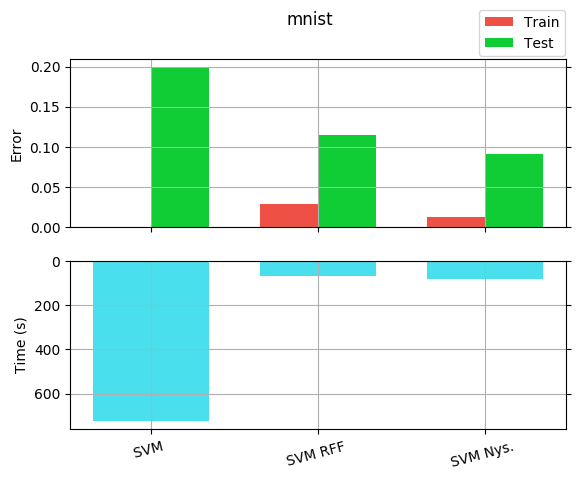
\includegraphics[width=\imgscale\linewidth]{Figures/\filePrefix/mnist}
    \caption{Exp. 3.4 with MNIST. Black Box Models with Support Vector Machine. There is not much difference between Box Models}
    \label{fig:\undPrefix_mnist}
  \end{subfigure}
\end{figure}


\begin{figure}[ht]
  \centering
  \begin{subfigure}[t]{0.5\linewidth}
    \centering\captionsetup{width=.8\linewidth}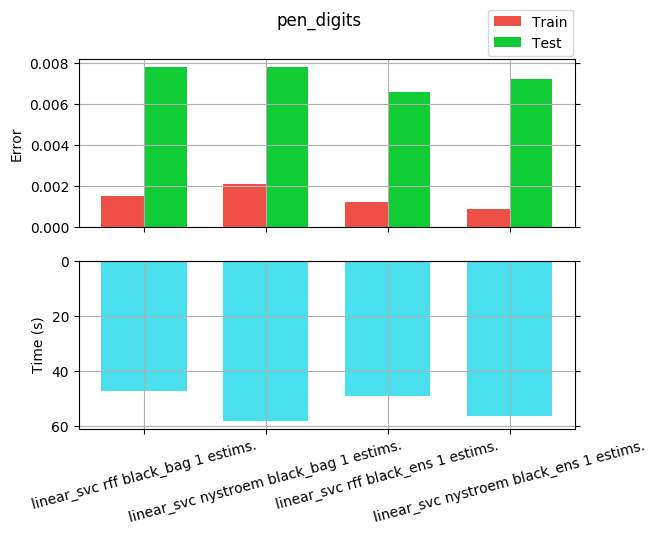
\includegraphics[width=\imgscale\linewidth]{Figures/\filePrefix/pen_digits}
    \caption{Exp. 3.4 with Pen Digits. Black Box Models with Support Vector Machine. There is not much difference between Box Models}
    \label{fig:\undPrefix_pen_digits}
  \end{subfigure}%
  \begin{subfigure}[t]{0.5\linewidth}
    \centering\captionsetup{width=.8\linewidth}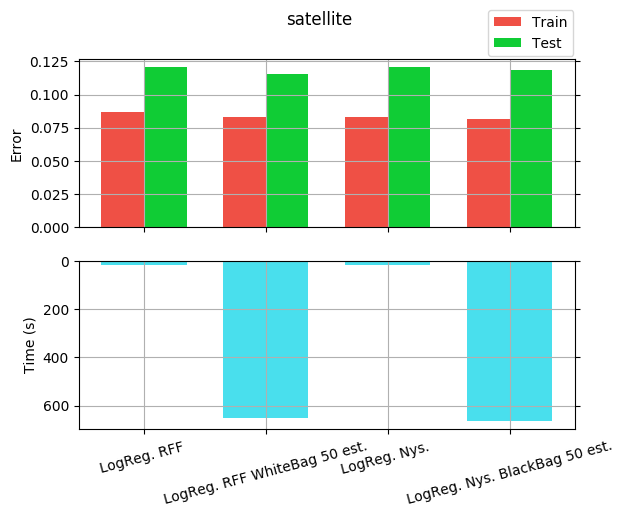
\includegraphics[width=\imgscale\linewidth]{Figures/\filePrefix/satellite}
    \caption{Exp. 3.4 with Satellite. Black Box Models with Support Vector Machine. There is not much difference between Box Models}
    \label{fig:\undPrefix_satellite}
  \end{subfigure}
\end{figure}

\begin{figure}[ht]
  \centering
  \begin{subfigure}[t]{0.5\linewidth}
    \centering\captionsetup{width=.8\linewidth}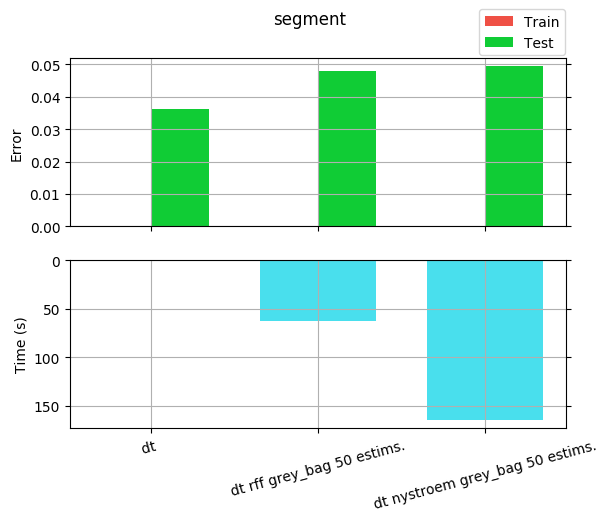
\includegraphics[width=\imgscale\linewidth]{Figures/\filePrefix/segment}
    \caption{Exp. 3.4 with Segment. Black Box Models with Support Vector Machine. There is not much difference between Box Models}
    \label{fig:\undPrefix_segment}
  \end{subfigure}%
  \begin{subfigure}[t]{0.5\linewidth}
    \centering\captionsetup{width=.8\linewidth}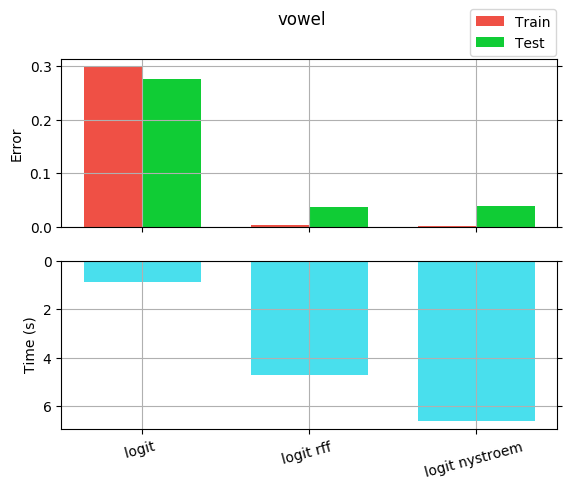
\includegraphics[width=\imgscale\linewidth]{Figures/\filePrefix/vowel}
    \caption{Exp. 3.4 with Vowel. Black Box Models with Support Vector Machine. There is not much difference between Box Models}
    \label{fig:\undPrefix_vowel}
  \end{subfigure}
\end{figure}


\begin{figure}[ht]
  \centering
  \begin{subfigure}[t]{0.5\linewidth}
    \centering\captionsetup{width=.8\linewidth}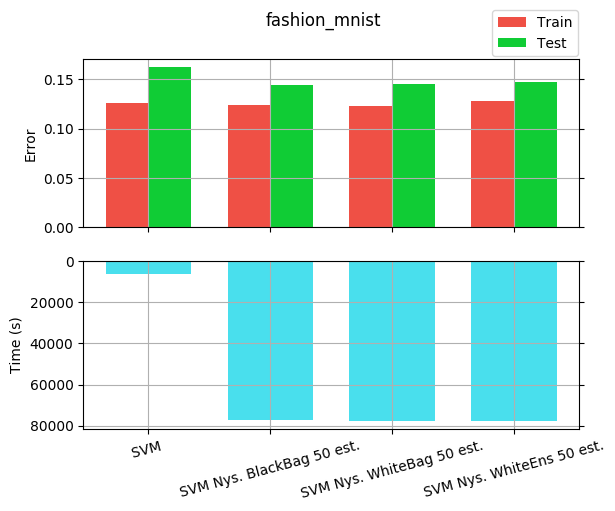
\includegraphics[width=\imgscale\linewidth]{Figures/\filePrefix/fashion_mnist}
    \caption{Exp. 3.4 with Fashion MNIST. Black Box Models with Support Vector Machine. There is not much difference between Box Models}
    \label{fig:\undPrefix_segment}
  \end{subfigure}%
\end{figure}


\let\major\undefined
\let\minor\undefined

\let\undPrefix\undefined
\let\dotPrefix\undefined
\let\scoPrefix\undefined

\let\filePrefix\undefined
